\begin{figure}[h]
    \centering
    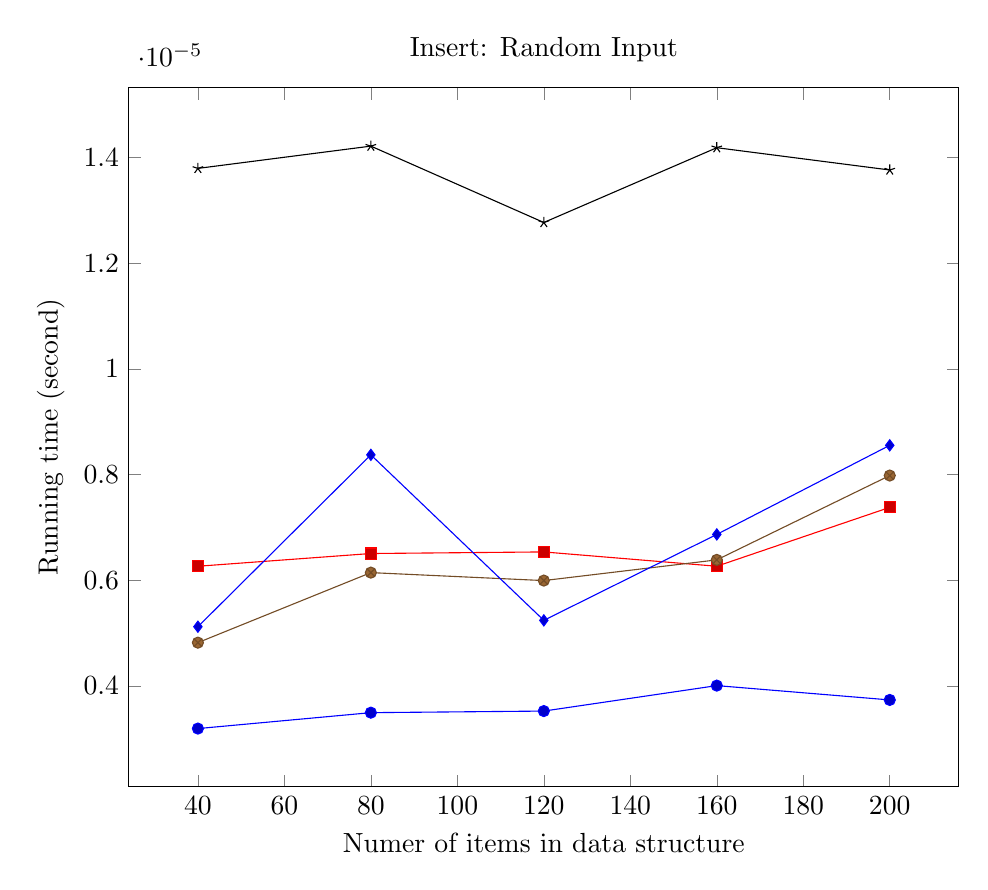
\begin{tikzpicture}
        \begin{axis}[
            xlabel={Numer of items in data structure},
            ylabel={Running time (second)},
            title={Insert: Random Input},
            width=\textwidth
        ]
		\addplot coordinates {
			(40, 3.1924585695009e-06)
			(80, 3.4936339062596743e-06)
			(120, 3.523751439971079e-06)
			(160, 4.00563197864301e-06)
			(200, 3.7345741755956397e-06)
		};
		\addplot coordinates {
			(40, 6.264447004511453e-06)
			(80, 6.505387273847419e-06)
			(120, 6.535504807558823e-06)
			(160, 6.264447004511453e-06)
			(200, 7.378795750412337e-06)
		};
		\addplot coordinates {
			(40, 4.818805388140391e-06)
			(80, 6.1439768700211065e-06)
			(120, 5.993389201108812e-06)
			(160, 6.3849171390018e-06)
			(200, 7.981146423574614e-06)
		};
		\addplot coordinates {
			(40, 1.3793830423125541e-05)
			(80, 1.4215475894729935e-05)
			(120, 1.2769834278358871e-05)
			(160, 1.418535836101853e-05)
			(200, 1.3763712889769408e-05)
		};
		\addplot coordinates {
			(40, 5.1199807248991645e-06)
			(80, 8.372674361822874e-06)
			(120, 5.240450859389511e-06)
			(160, 6.866797678029002e-06)
			(200, 8.55337956373603e-06)
		};
        \legend{}
        \end{axis}
    \end{tikzpicture}
    \caption{Average of 0 operations, benchmarked every 0, starting at 0.}
\end{figure}